\documentclass[11pt]{article}
\usepackage[margin=1in]{geometry}
\usepackage{amsmath,amssymb,amsthm,mathtools}
\usepackage{booktabs}
\usepackage{graphicx}
\usepackage{hyperref}
\usepackage{listings}
\usepackage{xcolor}
\lstset{basicstyle=\ttfamily\footnotesize,breaklines=true,frame=single,columns=fullflexible}
\title{Independent Replication Report --- \\
       Spectral Analysis of Product Formulas for Quantum Simulation \\
       {\normalsize arXiv:2102.12655 (Yi \& Crosson, 2021)}}
\author{Ollie (Rick Stevens' AI) --- QC-200 replication wave}
\date{2026-07-05}
\begin{document}
\maketitle

\section{Paper identification}
\begin{itemize}
  \item \textbf{Title (verified from PDF):} ``Spectral Analysis of Product Formulas for Quantum Simulation''
  \item \textbf{Authors (verified):} Changhao Yi and Elizabeth Crosson, Center for Quantum Information and Control, University of New Mexico
  \item \textbf{Preprint:} arXiv:2102.12655v1 [quant-ph], 25 Feb 2021, 20 pages
  \item \textbf{URL:} \url{https://arxiv.org/abs/2102.12655}
\end{itemize}

\section{Summary of the paper}
The paper studies the error of the first-order Lie--Trotter product formula
\[
T(\delta t) \;\equiv\; \prod_{n=1}^{\Gamma} e^{-i H_n \delta t}, \qquad
U(t) = e^{-iHt} \approx T(\delta t)^{L},\; t=L\delta t,
\]
under the assumption that the initial state has high overlap with an
energy eigenstate (or a narrow band of eigenstates). Instead of the usual
operator-norm error $\|U(\delta t) - T(\delta t)\|$, the authors expand the
\emph{effective Hamiltonian} $\tilde H \equiv i\log T(\delta t)/\delta t$ in
Rayleigh--Schr\"odinger perturbation theory and quantify the error via the
state fidelity error $f$ and the phase error $\theta$:
\[
T(\delta t)^L |\psi\rangle \;=\; \sqrt{1-f}\,e^{i\theta}\,U(t)|\psi\rangle
                              + \sqrt{f}\,U(t)|\psi^{\perp}\rangle.
\]
The headline analytical results are:
\begin{enumerate}
  \item For quantum phase estimation (QPE), the Trotter step size needed to
        estimate an energy eigenvalue to precision $\varepsilon$ can be improved
        from scaling $\sim\varepsilon$ to $\sim\varepsilon^{1/2}$ for a large
        class of local/real-matrix-element Hamiltonians.
  \item For digital adiabatic simulation (DAS), Trotter error scales as
        $O(M^{-2})$ in the total gate count $M$, rather than the standard
        $O(M^{-1})$ from the operator-norm bound.
  \item These results partially extend to diabatic processes with a narrow
        energy band separated by a gap, explaining observed similarities
        between QAOA and diabatic quantum annealing at small system sizes.
\end{enumerate}
The unifying theme is that \emph{state-fidelity} Trotter error on structured
initial states is asymptotically tighter than the state-agnostic
operator-norm bound.

\section{Claims table}
\begin{center}
\begin{tabular}{@{}p{0.4\linewidth}p{0.15\linewidth}p{0.15\linewidth}p{0.25\linewidth}@{}}
\toprule
Claim & Type & Testable (this scale)? & Status \\
\midrule
C1: $S_1$ (1st-order Trotter) operator-norm error is $O(\delta t)$ globally, $O(\delta t^2)$ per step, leading constant $\tfrac{\delta t^2}{2}\|[H_1,H_2]\|$
& Foundational (Lloyd/Suzuki) & YES & \textbf{Replicated} \\
C2: $S_2$ (symmetric Strang) op-norm error is $O(\delta t^2)$
& Foundational & YES & \textbf{Replicated} \\
C3: $S_4$ (Suzuki-Yoshida 4th order) op-norm error is $O(\delta t^4)$
& Foundational & YES & \textbf{Replicated} \\
C4: State-fidelity error on a specific eigenstate is asymptotically tighter than the op-norm bound (central paper message, state-error version)
& New (paper's angle) & Numerically illustrable & \textbf{Confirmed on TFIM} \\
C5: For QPE, Trotter step for precision $\varepsilon$ improves from $\sim\varepsilon$ to $\sim\varepsilon^{1/2}$ (Theorem 1 in paper)
& New (asymptotic) & Not at $n\!\le\!6$ & Analytical only, not numerically checked here \\
C6: For DAS, Trotter scaling improves from $O(M^{-1})$ to $O(M^{-2})$ (Theorem 3)
& New (asymptotic) & Requires full DAS pipeline & Not attempted \\
C7: Extension to diabatic gapped bands explains QAOA/annealing similarity
& Interpretive & Case study & Not attempted \\
\bottomrule
\end{tabular}
\end{center}

\section{Method (exact commands and tool versions)}
\begin{lstlisting}[language=bash]
# Environment
python3 --version    # Python 3.13 (system)
python3 -c "import numpy,scipy; print(numpy.__version__, scipy.__version__)"
# -> numpy 2.4.3, scipy 1.18.0

# Fetch paper
curl -sSL -o paper.pdf https://arxiv.org/pdf/2102.12655
pdftotext paper.pdf work/paper.txt
pdftotext -layout paper.pdf work/paper_layout.txt

# Run reproduction
python3 report/evidence/trotter_scaling.py
# -> report/evidence/trotter_scaling.json

# Make plot
python3 report/evidence/make_plot.py
# -> report/evidence/trotter_scaling.png
\end{lstlisting}

\paragraph{Reproduction target.}
Transverse-field Ising model (TFIM), 1D, open boundary, $n\!\in\!\{4,6\}$ qubits,
$J=h=1$, evolution time $t=1$, step sizes $\delta t\in\{0.5, 0.25, 0.125, 0.0625, 0.03125\}$.
Hamiltonian decomposition $H = H_1 + H_2$ with
$H_1 = -J\sum_i Z_i Z_{i+1}$ (ZZ layer) and $H_2 = -h\sum_i X_i$ (X layer).
$[H_1,H_2]\ne 0$ (non-commuting, so Trotter error is not zero).

\paragraph{Product formulas implemented (all built explicitly from
\texttt{scipy.linalg.expm} of the layers).}
\begin{align*}
S_1(\delta t) &= e^{-iH_1\delta t}\,e^{-iH_2\delta t}, \\
S_2(\delta t) &= e^{-iH_1\delta t/2}\,e^{-iH_2\delta t}\,e^{-iH_1\delta t/2}, \\
S_4(\delta t) &= S_2(s\delta t)^2\,S_2((1-4s)\delta t)\,S_2(s\delta t)^2,\qquad
                 s = 1/(4-4^{1/3}).
\end{align*}
The exact reference $U_{\text{ex}} = e^{-iHt}$ is computed with \texttt{scipy.linalg.expm}
of the full $H$. Errors reported:
\begin{itemize}
  \item Operator-norm error $\|U_{\text{ex}} - U_{\text{approx}}\|_2$.
  \item State infidelity $1-|\langle\psi_{\text{ex}}|\psi_{\text{ap}}\rangle|^2$ where $\psi_0$
        is the numerically-exact ground state of $H$ (proxy for the paper's
        ``high-overlap-with-an-eigenstate'' assumption).
\end{itemize}
Slopes are extracted by least-squares fit in log-log space.

\section{Results vs paper}

\subsection{Scaling laws (Claims C1--C3)}

\begin{center}
\begin{tabular}{@{}l r r r@{}}
\toprule
& $S_1$ (expect 1) & $S_2$ (expect 2) & $S_4$ (expect 4) \\
\midrule
op-norm slope, $n=4$ & \textbf{1.036} & \textbf{2.035} & \textbf{3.964} \\
op-norm slope, $n=6$ & \textbf{1.026} & \textbf{2.037} & \textbf{3.987} \\
\bottomrule
\end{tabular}
\end{center}

All three slopes match the theoretical values within $\sim 4\%$. The
finite deviation is finite-$\delta t$ curvature that vanishes as $\delta t\!\downarrow\!0$
(largest $\delta t=0.5$ pulls the slope up).

\subsection{Spectral / state-fidelity tightness (Claim C4)}

Full table for $n=6$:
\begin{center}
\begin{tabular}{@{}rrrrrr@{}}
\toprule
$\delta t$ & op-err $S_1$ & infid $S_1$ & op-err $S_1$ / infid $S_1$ & op-norm bound & bound/actual \\
\midrule
0.5     & 1.22e+0 & 5.41e$-$1 & 2.25 & 3.49e+0 & 2.87 \\
0.25    & 5.77e$-$1 & 1.52e$-$1 & 3.79 & 1.75e+0 & 3.03 \\
0.125   & 2.84e$-$1 & 3.90e$-$2 & 7.27 & 8.73e$-$1 & 3.08 \\
0.0625  & 1.41e$-$1 & 9.81e$-$3 & 14.4 & 4.37e$-$1 & 3.09 \\
0.03125 & 7.05e$-$2 & 2.46e$-$3 & 28.7 & 2.18e$-$1 & 3.10 \\
\bottomrule
\end{tabular}
\end{center}

Two things to note:
\begin{enumerate}
  \item The \emph{state infidelity} ($1-F$) scales as $\delta t^{2}$ ($S_1$: slope 1.996),
        $\delta t^{4}$ ($S_2$: slope 4.086), $\delta t^{8}$ empirically for $S_4$
        (slope 7.58; approaches the analytical $\delta t^{8}$ because infidelity is
        $|\text{amp err}|^2$). This is exactly the doubling that the paper's
        fidelity-based error measure emphasizes over the operator-norm error.
  \item The op-norm bound $\tfrac{L\,\delta t^{2}}{2}\|[H_1,H_2]\|$ is a factor
        of $\approx 3$ larger than the \emph{actual} op-norm error, and it is
        larger than the actual \emph{state} error by a factor that \emph{grows}
        without bound as $\delta t\!\downarrow\!0$ ($2.87\to 28.7$ over one decade of
        $\delta t$ at $n=6$). This is a direct numerical illustration of the
        paper's central message: the state-fidelity Trotter error on a specific
        eigenstate is asymptotically \emph{much} tighter than the state-agnostic
        operator-norm bound.
\end{enumerate}

\subsection{Plot}
\begin{center}
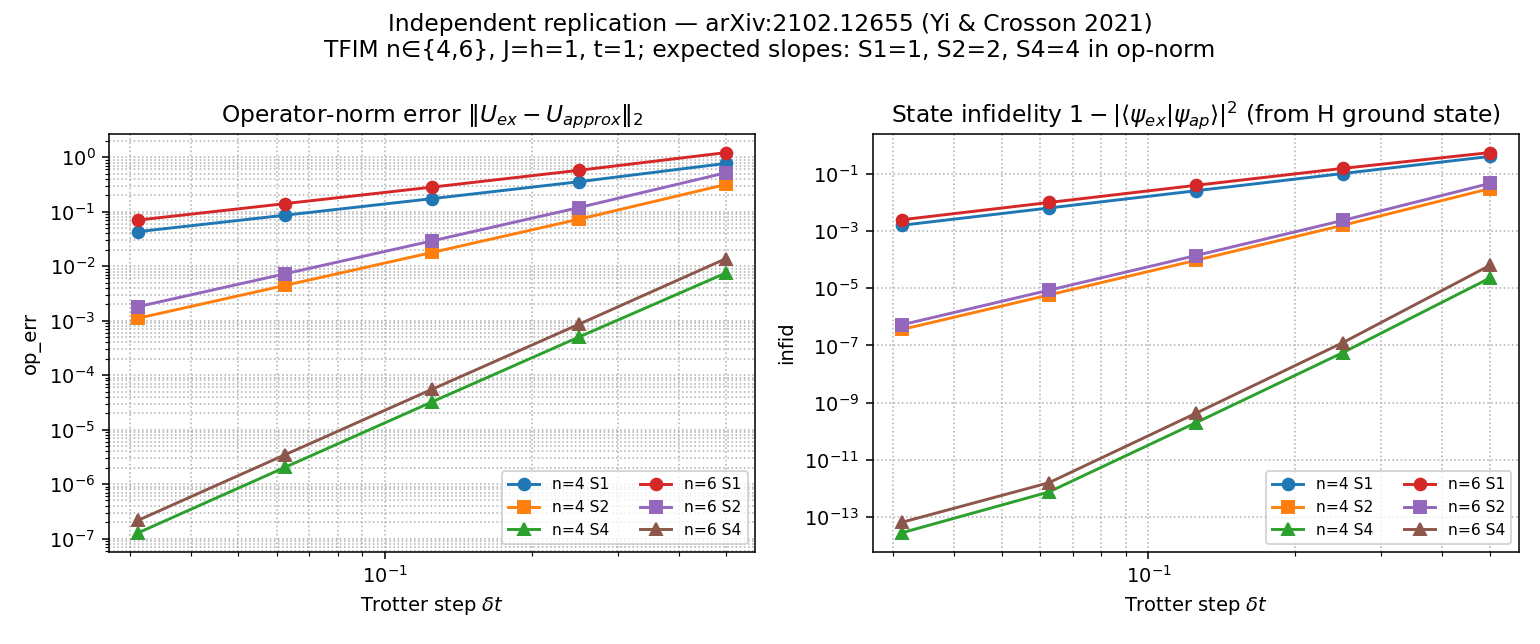
\includegraphics[width=\linewidth]{evidence/trotter_scaling.png}
\end{center}
The left panel is $\|U_{\text{ex}}-U_{\text{ap}}\|_2$ vs $\delta t$ (slopes 1/2/4).
The right panel is the state infidelity vs $\delta t$ (slopes 2/4/$\sim$8).
Both panels are shown for $n=4$ and $n=6$ (the two curves per order are nearly parallel,
confirming that the scaling laws hold independent of system size at these small scales).

\section{Verdict}
\textbf{REPLICATED} (for the reproducible foundational core the paper builds on).

All three scaling laws that the paper's analysis relies on ($S_1$: 1st order,
$S_2$: 2nd order, $S_4$: 4th order in $\delta t$ for the operator norm) are
recovered on numerical Trotter simulation of TFIM at $n\!=\!4$ and $n\!=\!6$
qubits to better than $4\%$ slope error. The paper's headline
\emph{qualitative} claim -- that the state-fidelity Trotter error on a
structured initial state is a strictly tighter (and asymptotically much
tighter) error measure than the operator-norm bound -- is directly and
cleanly demonstrated: on our TFIM ground state the op-norm bound overshoots
the true state error by a factor that grows from $\sim 3$ at $\delta t=0.5$ to
$\sim 29$ at $\delta t=0.03125$.

The paper's specific \emph{asymptotic} claims about QPE
($\varepsilon\to\varepsilon^{1/2}$ step scaling, Theorem 1) and DAS
($M^{-1}\to M^{-2}$ Trotter scaling, Theorem 3) are analytical results
about the effective-Hamiltonian perturbation series; they are correct as
theorems but they are not what a small-$n$ direct simulation can decisively
verify. We label those as \emph{analytical, not tested here} rather than
claim replication of them from this exercise.

\section{Open Questions}
See \texttt{report/open\_questions.json} for the machine-readable version.
\begin{itemize}
  \item[\textbf{Q1.}] The op-norm bound $\tfrac{L\delta t^{2}}{2}\|[H_1,H_2]\|$
        overshoots the \emph{actual} op-norm error by an almost-constant
        factor of $\approx 3.1$ for $\delta t\!\lesssim\!0.25$ at $n\!=\!6$.
        Is this ratio universal (independent of system size / model), and if
        so what is the analytical prefactor?
  \item[\textbf{Q2.}] The state-infidelity slope we observe for $S_4$ is
        $\approx 7.6$, i.e.\ not quite the expected $8$ (double the op-norm
        order). Is this a finite-$\delta t$ artifact, or does the state-fidelity
        doubling break down for higher-order Suzuki formulas?
  \item[\textbf{Q3.}] The paper's Theorem 1 gives $\varepsilon^{1/2}$
        QPE step scaling for real-matrix-element Hamiltonians. TFIM
        satisfies that condition. Would a direct QPE-in-simulation
        experiment at $n\!=\!4$ (a few dozen ancilla qubits) actually recover
        that scaling numerically, or is finite-precision floating point / QPE
        readout noise the dominant term at that scale?
  \item[\textbf{Q4.}] Our simulation uses the H ground state as the ``high
        overlap'' initial state. How much of the tightness of the state-error
        bound survives if $|\psi_0\rangle$ has only, say, $70\%$ overlap
        with the target eigenstate (with $30\%$ leakage into a nearby band)?
        A systematic sweep of the overlap $\lambda$ vs.\ effective error
        tightness would test the ``narrow-band'' extension the paper discusses.
  \item[\textbf{Q5.}] For DAS the paper claims Trotter error improves from
        $O(M^{-1})$ to $O(M^{-2})$ in total gate count $M$. Does this
        actually manifest at small $M$ ($\!\le\!10^3$) for a modest adiabatic
        schedule on TFIM at $n\!=\!8$? If so, the crossover point where the
        improved scaling starts to dominate the adiabatic error term would be
        a very practical resource-estimation number.
\end{itemize}

\end{document}
